% fix-cm makes the Computer Modern maths fonts scale to any size.
\RequirePackage{fix-cm}
\documentclass[tikz,border=6pt]{standalone}
% Shared style for the method diagrams in this folder.
% Each diagram is a standalone document that loads fix-cm, then
% \documentclass[tikz,border=6pt]{standalone}, then inputs this file.
% scripts/build_diagrams.sh compiles every diagram except this file, once
% for the light theme and once with \darkmode defined for the dark theme.

\usepackage[T1]{fontenc}
\usepackage[scaled=0.95]{helvet}
\renewcommand{\familydefault}{\sfdefault}
\usepackage{amsmath,amssymb}
\usetikzlibrary{arrows.meta,positioning,calc,shapes.misc}

% Method colours, matching the interactive page and docs/figures.
% Onsets are blue and reports orange, as in the logo.
\definecolor{bscol}{HTML}{2A78D6}
\definecolor{meancol}{HTML}{EB6834}
\definecolor{fwdcol}{HTML}{1BAF7A}
\definecolor{gencol}{HTML}{EDA100}
\definecolor{onsetcol}{HTML}{2A78D6}
\definecolor{reportcol}{HTML}{EB6834}

% Theme colours, as in docs/figures/make_figures.py. `paper` is the page
% background, used for label backgrounds and tinted fills.
\ifdefined\darkmode
  \definecolor{ink}{HTML}{F2F2F0}
  \definecolor{textcol}{HTML}{D6D6D4}
  \definecolor{muted}{HTML}{9A9A97}
  \definecolor{gridcol}{HTML}{3A3A38}
  \definecolor{barcol}{HTML}{6A6A66}
  \definecolor{paper}{HTML}{1E2029}
  \def\tint{18}
\else
  \definecolor{ink}{HTML}{0B0B0B}
  \definecolor{textcol}{HTML}{333333}
  \definecolor{muted}{HTML}{6B6B6B}
  \definecolor{gridcol}{HTML}{E2E2DF}
  \definecolor{barcol}{HTML}{C4C4BF}
  \definecolor{paper}{HTML}{FFFFFF}
  \def\tint{9}
\fi

\color{textcol}

\tikzset{
  every node/.style={font=\small, text=textcol,
    execute at begin node={\thickmuskip=5mu\medmuskip=4mu\thinmuskip=3mu
      \hyphenpenalty=10000\exhyphenpenalty=10000}},
  panel/.style={rectangle, rounded corners=4pt, draw=#1, line width=0.9pt,
    fill=#1!\tint!paper},
  box/.style={rectangle, rounded corners=3pt, draw=#1, line width=0.8pt,
    fill=#1!\tint!paper, align=center, inner sep=5pt, minimum height=9mm},
  paneltitle/.style={font=\normalsize\bfseries, text=#1, anchor=north west,
    inner sep=0pt},
  flow/.style={-{Stealth[length=2.4mm,width=1.9mm]}, line width=0.9pt,
    draw=ink!80},
  axis/.style={line width=0.6pt, draw=muted},
  cutoff/.style={line width=0.8pt, draw=ink, dash pattern=on 2.5pt off 2pt},
  onset/.style={circle, fill=onsetcol, inner sep=0pt, minimum size=1.9mm},
  report/.style={rectangle, fill=reportcol, inner sep=0pt,
    minimum size=1.8mm},
  missing/.style={circle, draw=onsetcol, densely dotted, line width=0.7pt,
    inner sep=0pt, minimum size=1.9mm},
  link/.style={line width=0.6pt, draw=ink!55},
  bar/.style={fill=#1, draw=none},
  note/.style={font=\footnotesize, text=muted, align=center},
  label/.style={font=\footnotesize, text=textcol, inner sep=1.5pt},
  edgelabel/.style={font=\footnotesize, text=textcol, fill=paper,
    inner sep=1.5pt, align=center},
}

% The smallest text size. The figures are scaled to the page column, about
% 1.2 times their natural width, so 8.5 pt renders at about 13 px.
\renewcommand{\footnotesize}{\fontsize{8.5}{10.2}\selectfont}


% Top: EM with one delay per period of onset days, counted back from the
% cut-off, each shrunk towards the period before. Bottom: the steps of
% one nowcast sample. Here T = 27 and P = 8, so K = 4 and the first period
% is 4 days long. The delays are illustrative discretised Gammas with
% shape 2 and means 7, 6, 5 and 4 days.

\begin{document}
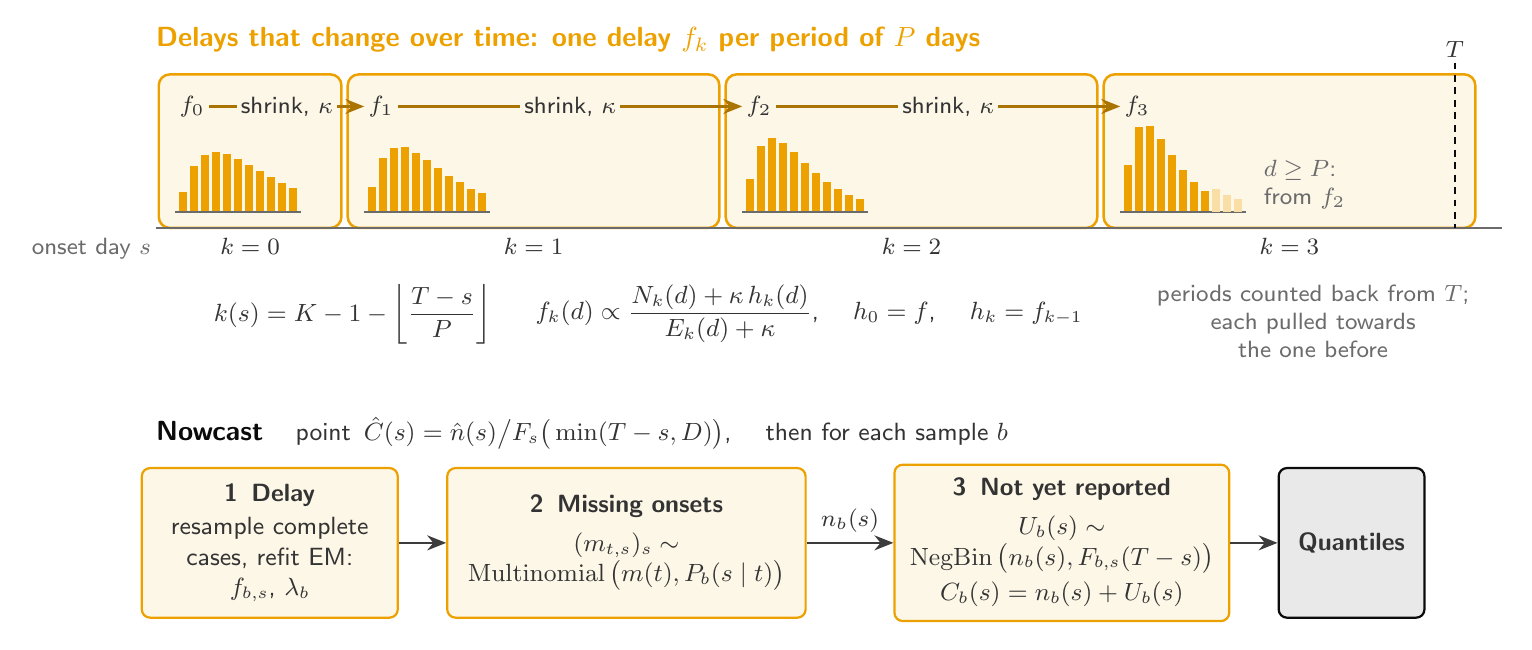
\begin{tikzpicture}[x=1cm,y=1cm]

% ---- Periods -------------------------------------------------------------
% Onset day s sits at x = 0.6 s.
\node[paneltitle=gencol] at (-0.3,0)
  {Delays that change over time: one delay $f_k$ per period of $P$ days};

\foreach \k/\a/\b in {0/0/3, 1/4/11, 2/12/19, 3/20/27} {
  \fill[panel=gencol] ({0.6*(\a-0.5)+0.04},-0.6) rectangle
    ({0.6*(\b+0.5)-0.04},-2.55);
  \node[label, anchor=north] at ({0.6*(\a+\b)/2},-2.62) {$k = \k$};
}

% #1 period, #2 first day, #3 bars as d/p.
\newcommand{\periodpmf}[3]{%
  \begin{scope}[shift={({0.6*(#2-0.5)+0.35},-2.35)}]
    \foreach \d/\p in {#3}
      \fill[bar=gencol] ({0.14*\d-0.05},0) rectangle ({0.14*\d+0.05},{6*\p});
    \draw[axis] (-0.1,0) -- (1.5,0);
    \node[label, anchor=south west] (f#1) at (-0.1,1.15) {$f_{#1}$};
  \end{scope}}
\periodpmf{0}{0}{0/0.043, 1/0.097, 2/0.121, 3/0.127, 4/0.123, 5/0.113,
  6/0.1, 7/0.087, 8/0.074, 9/0.062, 10/0.052}
\periodpmf{1}{4}{0/0.053, 1/0.114, 2/0.136, 3/0.137, 4/0.126, 5/0.11,
  6/0.093, 7/0.077, 8/0.063, 9/0.05, 10/0.04}
\periodpmf{2}{12}{0/0.07, 1/0.14, 2/0.156, 3/0.147, 4/0.127, 5/0.104,
  6/0.082, 7/0.064, 8/0.048, 9/0.036, 10/0.027}
\periodpmf{3}{20}{0/0.099, 1/0.18, 2/0.182, 3/0.155, 4/0.121, 5/0.089,
  6/0.064, 7/0.045}
% The latest period cannot show delays of P days or more by the cut-off,
% so it keeps the previous period's values there.
\begin{scope}[shift={({0.6*19.5+0.35},-2.35)}]
  \foreach \d/\p in {8/0.048, 9/0.036, 10/0.027}
    \fill[bar=gencol!35!paper] ({0.14*\d-0.05},0) rectangle
      ({0.14*\d+0.05},{6*\p});
  \node[note, anchor=west, align=left] at (1.6,0.35)
    {$d \ge P$:\\ from $f_2$};
\end{scope}

\foreach \a/\b in {0/1, 1/2, 2/3}
  \draw[flow, draw=gencol!70!ink] (f\a.east) -- (f\b.west)
    node[edgelabel, midway, fill=gencol!\tint!paper] {shrink, $\kappa$};

\draw[axis] (-0.3,-2.55) -- ({0.6*27.5+0.3},-2.55);
\draw[cutoff] ({0.6*27},-0.45) -- ({0.6*27},-2.55);
\node[label, anchor=south] at ({0.6*27},-0.45) {$T$};
\node[label, text=muted, anchor=north east] at (-0.3,-2.62) {onset day $s$};

\node[anchor=north] at (2.2,-3.15)
  {$k(s) = K - 1 - \left\lfloor \dfrac{T - s}{P} \right\rfloor$};
\node[anchor=north] at (8.0,-3.15)
  {$f_k(d) \propto \dfrac{N_k(d) + \kappa \, h_k(d)}{E_k(d) + \kappa}$,
   \quad $h_0 = f$, \quad $h_k = f_{k-1}$};
\node[note, anchor=north, text width=4.6cm] at (14.4,-3.15)
  {periods counted back from $T$;\\ each pulled towards the one before};

% ---- Nowcast -------------------------------------------------------------
\def\yh{-5.0}
\def\yr{-6.55}
\node[paneltitle=ink] (nt) at (-0.3,\yh) {Nowcast};
\node[anchor=base west, xshift=8pt] at (nt.base east)
  {point\enspace $\hat C(s) = \hat n(s) \big/ F_s\big(\min(T - s, D)\big)$,
   \quad then for each sample $b$};

\node[box=gencol, text width=2.9cm, minimum height=19mm] (b1)
  at (1.15,\yr)
  {\textbf{1\enspace Delay}\\[1pt] resample complete\\ cases, refit EM:\\
   $f_{b,s}$, $\lambda_b$};
\node[box=gencol, text width=4.2cm, minimum height=19mm, right=0.6cm of b1]
  (b2)
  {\textbf{2\enspace Missing onsets}\\[3pt] $(m_{t,s})_s \sim$\\
   $\operatorname{Multinomial}\big(m(t), P_b(s \mid t)\big)$};
\node[box=gencol, text width=3.9cm, minimum height=19mm, right=1.1cm of b2]
  (b3)
  {\textbf{3\enspace Not yet reported}\\[3pt] $U_b(s) \sim$\\
   $\operatorname{NegBin}\big(n_b(s), F_{b,s}(T - s)\big)$\\[2pt]
   $C_b(s) = n_b(s) + U_b(s)$};
\node[box=ink, text width=1.5cm, minimum height=19mm, right=0.6cm of b3]
  (q) {\textbf{Quantiles}};
\draw[flow] (b1) -- (b2);
\draw[flow] (b2) -- (b3)
  node[edgelabel, midway, above=2pt, fill=none] {$n_b(s)$};
\draw[flow] (b3) -- (q);

\end{tikzpicture}
\end{document}
